\chapter{Acceleration-Sensitive Interference}\label{chap:atom_int}
This chapter describes the work towards realising an atom interferometer and
subsequently measuring accelerations.
\section{Chapter Outline}
\verysubsection{To-Do}
\begin{itemize}
	\item Raman spectrum, identifying each transition
	\item Characterisation of velocity-selective pulse and each interferometer pulse using Rabi oscillations.
	\item Making a three-pulse atom interferometer
	\item Improving acceleration sensitivity and correlating vibrations using MEMS
\end{itemize}
\section{Raman Optical System}\label{sec:setup_ramanoptics}

When designing an optical system for the light used in an atom
interferometer, it is worth paying attention to both the spatial extent and
beam waist of the collimated beam. These requirements are particularly
important in this experiment, where acceleration due to gravity is
perpendicular to the Raman beam axis and causes significant transverse motion
of the atoms. Firstly, the optical system must be designed to make sure that
the atoms are illuminated by each interferometer pulse. In addition to this,
a more subtle requirement on the fringe contrast constrains the beam waist
size. The gradient of intensity across the atom cloud must be small so that
each atom is driven by (approximately) the same Rabi frequency. Otherwise,
this variation in the Rabi frequency will dephase the atoms, which reduces
the interferometer fringe contrast.
\par\noindent
A further constraint on the optical system comes from the effect of thickness
variation of optical elements. If the optical path length of the light as it
passes through an element is not uniform, this will lead to wavefront
aberrations. A spatially-varying phase leads to a bias in the interferometer
phase since it does not depend on acceleration. Moreover, since this phase is
not the same for each atom, it is another source of dephasing. Considering
the effects of wavefront aberrations was a large motivating factor for
designing an optical system for use inside the vacuum chamber. Specifically,
the distortions of a laser wavefront through optical viewports would
drastically reduce the fringe contrast under transverse motion of the atoms
during the interferometer. The process used to bond an optical viewport to a
flange stresses the glass and distorts its thickness, producing wavefront
aberrations that factor into the phase uncertainty of an atom
interferometer~\cite{Schkolnik2015}.
{\huge Add requirements on other optics}

\subsection{Fringe Contrast Dependence}\label{subsec:fringe_contrast}

The effects of a gradient of intensity on the fringe contrast can be shown by
considering an ensemble of atoms that are spatially distributed by a Gaussian
distribution. Neglecting the effect of the ensemble's velocity distribution
on the Raman detuning and for fixed pulse times, the pulse area \(\Omega
\tau\) varies only as a function of the radial displacement from the optic
axis. The total fringe contrast can be determined by a convolution of the
contrast for a single atom with the atomic density
\begin{equation}
	\mathcal{C} = \int \frac{1}{\sqrt{2\pi}\sigma_c}e^{-r^2/(2\sigma_c^2)} f_{\pi/2-\pi-\pi/2}\left(\Omega(r-r_1),\Omega_(r-r_2),\Omega(r-r_3)\right) \;\mathrm{d}r
	\label{eq:cloud_contrast}
\end{equation}
where \(\sigma_c\) is the radial width of the atom cloud,
\(f_{\pi/2-\pi-\pi/2}\) is the fringe contrast as previously described in
\EquationRef{eq:fringe_contrast} and \(r_i\) is the position of the
ensemble's centre-of-mass at the \(i\)-th pulse. If the atom cloud is
initially at the centre of the laser and falling under gravity, then these
coordinates are \(\left(0, -\frac{1}{2}g T^2, -2 g T^2\right)\) respectively.
Under the assumption that the two lasers which drive the Raman transition
have the same waist size, the Rabi frequency, which is determined by the
product of the electric fields (see~\EquationRef{eg:raman_rabi}), can be
described by
\begin{equation}
	\Omega(r) = \Omega_0 e^{-2 r^2/w^2}
\end{equation}
where \(\Omega_0\) is the Rabi frequency along the optic axis and \(w\) is
the waist size -- the distance at which the electric field falls to \(1/e\)
of its peak value. The fringe contrast as a function as beam waist for an
atom cloud of width a width \(\sigma_c = \sivalue{5}{\milli\metre}\) and a
time between interferometer pulses of \(T = \sivalue{25}{\milli\second}\) is
plotted in \FigureRef{fig:raman_fringecontrast}. For small beam waists, the
intensity gradient across the cloud significantly reduces the fringe
contrast. In fact, a beam waist much greater than the width of the cloud is
necessary to achieve a large contrast between the two interferometer states.
Relaxing the assumptions made on the ensemble's velocity distribution to
include its influence on the detuning and spatial distribution of the atoms
during the interferometer would strengthen this argument.
\begin{figure}[!ht]
	\centering
	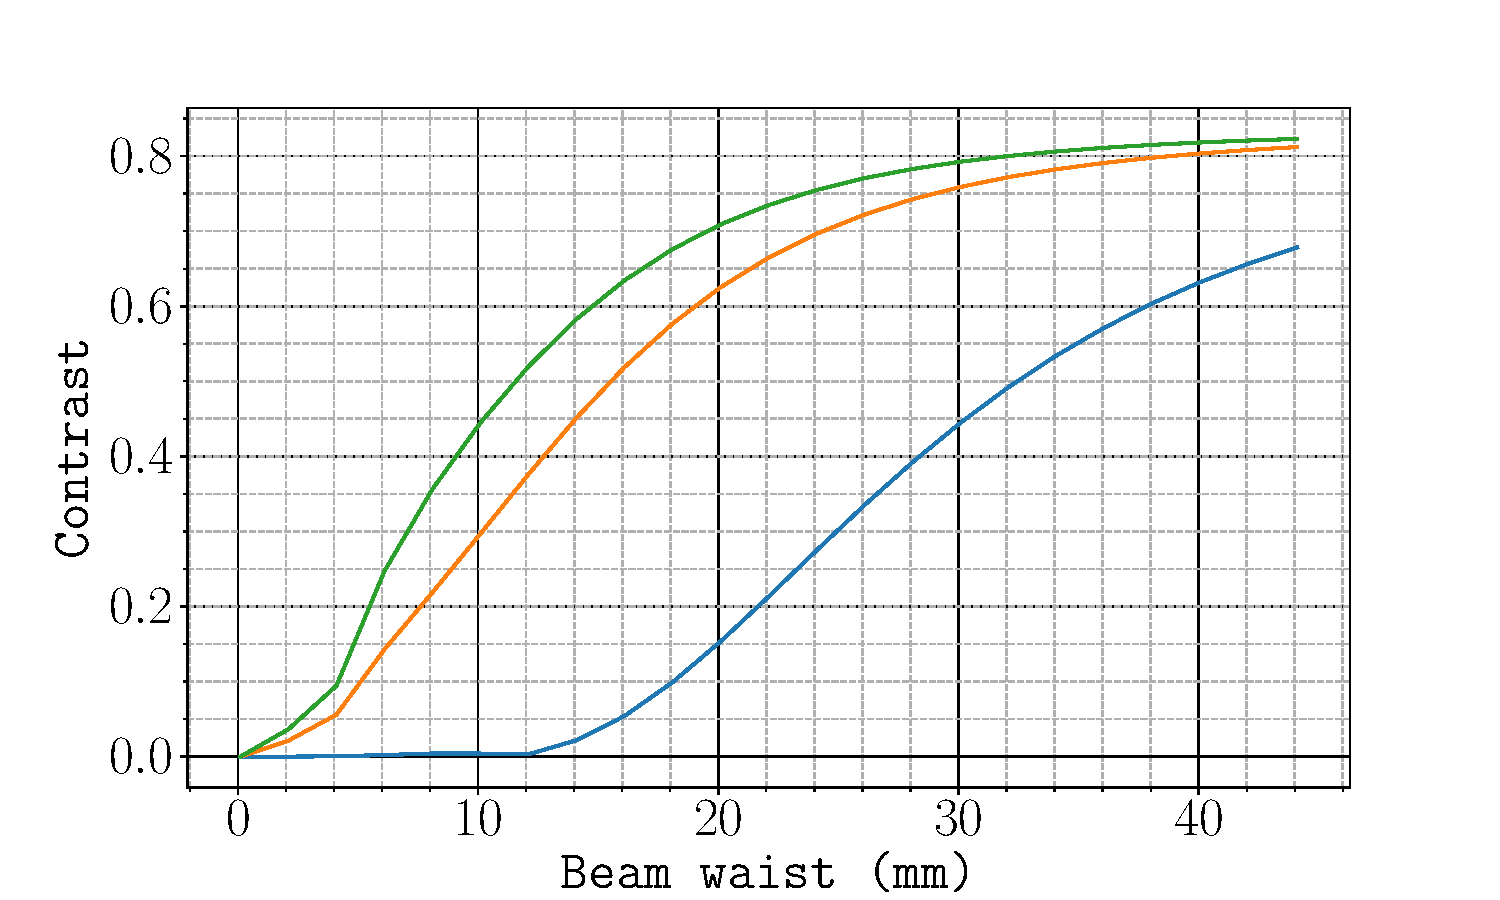
\includegraphics[width=0.5\textwidth]{fringe_contrast.pdf}
	\caption[Simulated fringe contrast vs beam waist size]{Simulated fringe
		contrast as a function of waist size \(w\) for an atom cloud falling under
		gravity. This model assumes a Gaussian distributed atomic density with a
		width \(\sigma_c = \sivalue{5}{\milli\metre}\) and a time between
		interferometer pulses of \(T = \sivalue{25}{\milli\second}\). For smaller
		beam waists the subsequent interferometer pulses have a larger intensity
		gradient across the atom ensemble, which increases the dephasing of the two
		states and reduces the interferometer fringe contrast.}
	\label{fig:raman_fringecontrast}
\end{figure}

So far, it has been shown that a large beam waist is necessary to achieve a
high fringe contrast when allowing for transverse motion of the atoms across
the laser wavefront. Otherwise, if the fringe contrast was poor, this would
limit the sensitivity of the interferometer to accelerations rather than
other effects which are less rectifiable. Another optical effect which
influences the sensitivity is distortions of the laser wavefront. In an ideal
case, the superposition of the spherical wavefronts of the two lasers results
in a planar wavefront for the effective field which drives the Raman
transition. However, propagation through rough optical elements distort these
wavefronts and introduce a spatially varying component of the Raman phase
that is independent of acceleration. If the atom cloud's trajectory is
parallel with the Raman axis, then this additional phase is the same at each
laser pulse and is therefore cancelled out. Of course, this does not occur
when the cloud moves transverse to the Raman axis where this random phase has
the effect of reducing the fringe contrast. Starting with the assumption that
this phase is Gaussian distributed around 0, with a standard deviation of
\(\sigma_\phi\), if this is uncorrelated at each interferometer pulse, then
the interferometer phase \(\Delta \Phi\) will be distributed with a standard
deviation of \(\sigma_\Phi = \sqrt{6} \sigma_\phi\). Denoting this random
phase as \(\delta\phi\), the fringe contrast is then given by
\begin{equation}
	\mathcal{C}(\delta \phi) = \cos\left(2 \delta\phi\right)
\end{equation}
Following from this, if \( \delta \phi\) is uncorrelated between each atom,
the expected value of the contrast over the ensemble is given by
\begin{align}
	\langle \mathcal{C} \rangle & = \frac{1}{\sqrt{2\pi}\sigma_\Phi}\int \mathcal{C}(\delta \phi) \; e^{-\delta\phi^2/2\sigma_\Phi^2} \; \mathrm{d}\delta\phi \\
	                            & = e^{-2 \sigma_\Phi^2}
\end{align}
The value of this expected contrast is plotted in
\FigureRef{fig:raman_phasenoise} and shows a strong dependence on
\(\sigma_\phi\).
{\huge Add more justification here. Cite Achim Peter's paper}
\begin{figure}
	\centering
	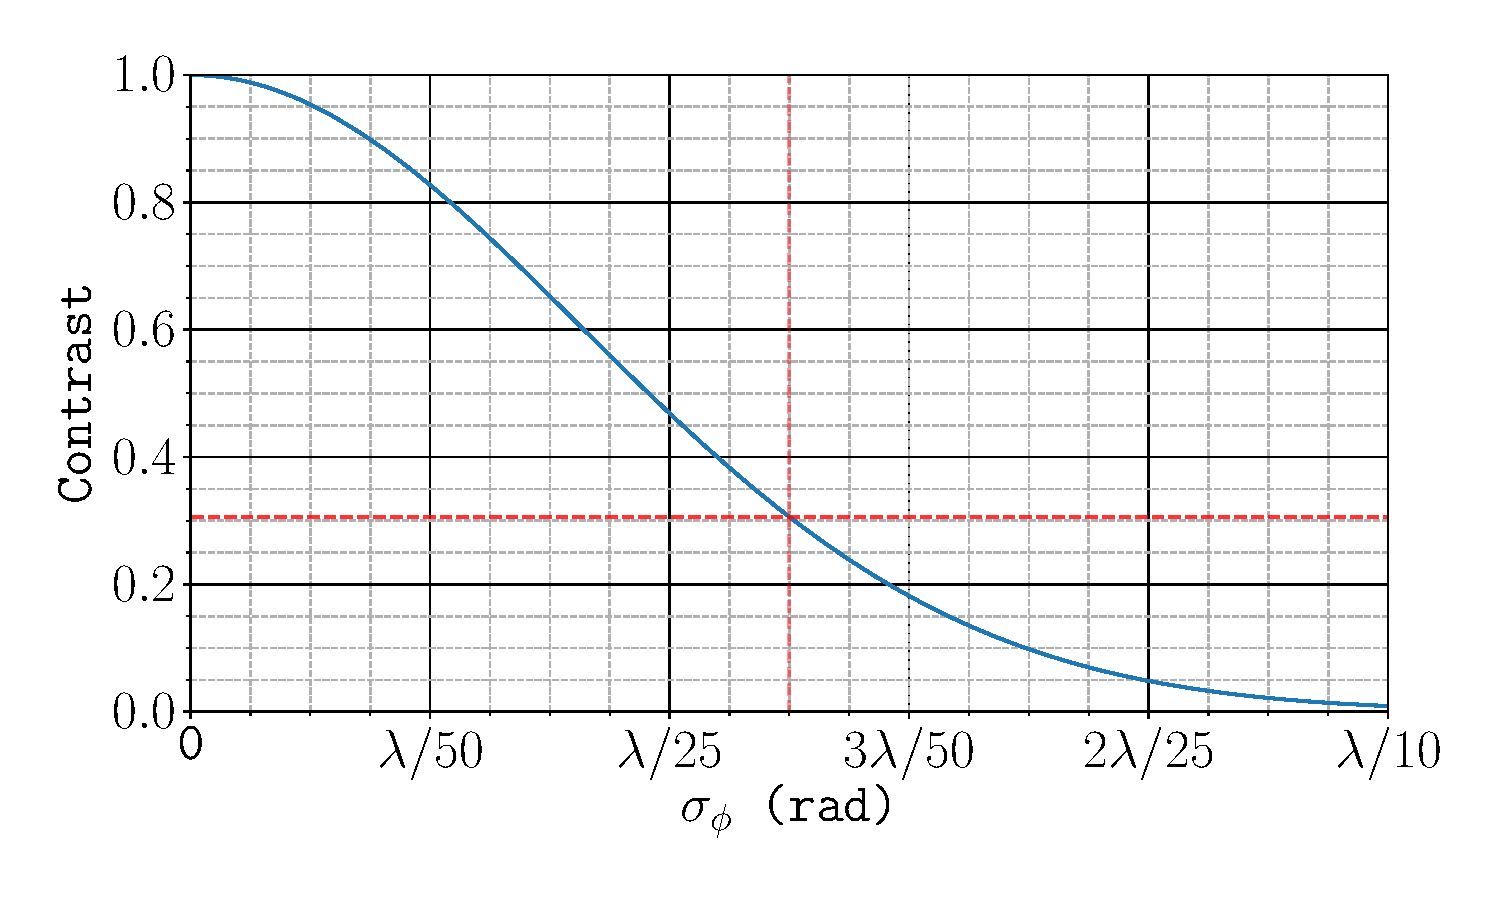
\includegraphics[width=0.5\textwidth]{phase_noise_contrast.pdf}
	\caption{Expected contrast as a function of random phase contributions. This
		assumes that the phase imprinted on an atom during each interferometer pulse
		has an additional random component that is Gaussian distributed around 0 with
		a standard deviation of \(\sigma_\phi\). This random phase is also
		uncorrelated between each pulse so that the total can be obtained using
		Gaussian propagation of error. The dashed lines indicate the contrast for
		phase noise expected from conventional optics, which are usually engineered
		to a surface flatness of \(\lambda/20\).}
	\label{fig:raman_phasenoise}
\end{figure}
\subsection{Raman Beam Collimator}\label{subsec:setup_ramancollimator}
The optical system used to produce the beams for driving Raman transitions,
which will conventionally be referred to as the Raman optics, was designed to
reduce the previously mentioned effects which result in poorer
interferometric fringe visibility and sensitivity to accelerations.
Principally, the entire optical system was mounted inside the optical chamber
so that the Raman light does not pass through any optical viewports before
interacting with the atoms. Typically, the stress placed on the glass during
the bonding process will distort the flatness more than is acceptable for
achieving a high contrast. For example the viewports used for the \ac{mot}
optics have a specified flatness of \(\lambda/4\), so mounting the entire
optical system inside the chamber was the simplest way to avoid a large
distortion. \par\noindent
\FigureRef{fig:raman_collimator} presents a diagram of the components used to
send Raman light into the chamber and produce a collimated beam in the centre
of the chamber. The light is coupled into the chamber using a UHV compatible
\ac{pm} fibre, manufactured by Diamond photonics. This is a kapton-coated
PM-780 HP fibre that is bonded on one end to a DN16 flange using an epoxy
resin. The external side of this flange has an FC/APC connector for coupling
light from another fibre. Inside the chamber, the ferrule is connected to an
FC/APC fibre plate. This is clamped between a piece which bolts onto the
inside of a DN63 flange and another stainless steel plate which bolts onto
the rest of the optics assembly. Fine adjustment of the position of the fibre
along the optic axis is achieved using shim plates with a thickness ranging
from 200--\sivalue{300}{\micro\metre}. The fibre plate is free to rotate so
that the orientation of the fibre with respect to a \ac{qwp} at the output of
the collimator. This \ac{qwp} is manufactured by Light Machinery, and is
described further is \SectionRef{subsec:setup_ramanmirror}. When the fibre is
correctly orientated (e.g. when the slow axis of the fibre is at 45\(\deg\)
to the slow axis of the waveplate), the two Raman light fields are
orthogonally circularly polarised. \par\noindent
The original design for the optical system consisted of a triplet lens, as a
system of three lenses is capable of correcting for the five types of Seidel
aberrations that distort rays of monochromatic light. This was designed and
manufactured by IC Optical Systems. Another specification for this lens
system was that it had to produce a collimated beam with a waist size of
around \sivalue{35}{\milli\metre} so that the sensitivity of the
interferometer was not limited by the effects of intensity gradients across
the atoms. Unfortunately, the triplet was designed with an incorrect \ac{na}.
With a focal length of \sivalue{123.4}{\milli\metre} and a diameter of
\sivalue{50}{\milli\metre}, the triplet lens has a \ac{na} of 0.194. However,
the nominal \ac{na} for PM780-HP fibre used in the UHV compatible \ac{pm}
fibre is 0.12. Consequently, the light from this fibre did not fill the
\ac{na} of the triplet lens and produced a beam with a waist of 13mm. {\huge
Plot to illustrate this}. To address this issue, a pair of aspheric lenses
was included to increase the divergence angle of light from the fibre. These
are manufactured by Thorlabs and have a focal length of
\sivalue{4.51}{\milli\metre} (352230-B) and \(\sivalue{15.29}{\milli\metre}\)
(352260-B), respectively, to give a magnification of 3.39.
\begin{figure}
	\centering
	\def\svgwidth{\columnwidth}
	\subfloat[][]{\scalebox{0.4}{\input{Figures/Chapter6/raman_optics.pdf_tex}\label{fig:raman_collimator}}}
	\subfloat[][]{\scalebox{0.4}{\input{Figures/Chapter6/mirror_mount.pdf_tex}\label{fig:mirror_mount}}}
	\caption[Drawings of the compenets used in the Raman optics
		assemblies]{Diagrams of the componets used in the Raman optical assemblies.
		(a) shows the collimator setup. Light is coupled into the chamber using a UHV
		fibre feedthrough. A pair of aspheric lenses is used to increase the
		divergence angle of the fibre output, before the light is collimated by a
		triplet lens. Finally, a quarter-wave plate is aligned so that it circularly
		polarises the collimated light fields. (b) illustrates the other half of the
		setup, which is used to retro-reflect the light. A second quarter-wave plate
		is used so that the reflected beams have the same handedness to their
		respected incoming ones. A MEMS accelerometer is mounted on the back of the
		mirror to measure vibrations. These components are all mounted on a
		piezo-controlled mirror mount whose tilt can be controlled from outside the
		vacuum chamber.}
	\label{fig:raman_optics}
\end{figure}
\subsubsection{Alignment and Collimation}
As one of the main motivations for mounting the Raman optics inside the
vaccuum chamber was to reduce the effects of wavefront distortions, it is
worth highlighting how inaccurate alignment of the optics can lead to
aberrations. As discussed before (see \SectionRef{subsec:fringe_contrast}),
distortions of the wavefront leads to a dephasing and loss of interferometer
fringe visibility. Here, the same figures of merit as before are used to
consider what misalignment is acceptable to ensure that the phase of the
Raman wavefront deviates by less than \(\lambda/100\) after a transverse
distance of \sivalue{12.5}{\milli\metre}. \par\noindent
Taking the fibre as a point source, misalignment can occur if it is displaced
from the front focal point of the optical system longitudinally along or
transversely to the optic axis. If it is transversely displaced, this
manifests as an angular displacement of the collimated light after the
triplet lens. A large angular displacement is undesirable due to the fact
that since one of the Raman light fields propagates further, the two
wavefronts that drive acceleration-sensitive Raman transitions are not
parallel. \FigureRef{fig:raman_wave_transverse} shows a simulation of the
wavefront distortion as a result of this transverse misalignment. This is
obtained by simulating the propagation of rays corresponding to each Raman
light field through the optical system. The wavefront is estimated using the
slope of each ray at a distance of \sivalue{43}{\milli\metre} from the output
of the triplet lens, which corresponds to the position of the centre of the
vacuum chamber. The mirror is mounted at the same distance from the centre,
so the second beam propagates \sivalue{129}{\milli\metre}. Close to the optic
axis, this distortion is approximately linear (i.e. a tilt) and it can be
seen that a displacement of the fibre from the optic axis of
<\sivalue{1}{\milli\metre} is sufficient to achieve the desired wavefront
flatness.
\par\noindent
Aside from a transverse displacement, it is possible that the fibre could be
misaligned along the optic axis. In which case, the output beam will not be
collimated. Consequently, the counter-propagating reflected rays will not be
antiparallel to incoming ones. The effect of this longitudinal displacement
on the Raman wavefront is shown in~\FigureRef{fig:raman_wave_longitudinal}.
Further from the optic axis the deviation in the phase of the light is
greater, giving a quadratic distortion which is characteristic of a defocus.
Comparing the wavefront distortion in this case, a requirement on the
longitudinal misalignment of \(< \sivalue{0.6}{\milli\metre}\) is needed for
the previously specified flatness.

\begin{figure}
	\centering
	\def\svgwidth{\columnwidth}
	\subfloat[][]{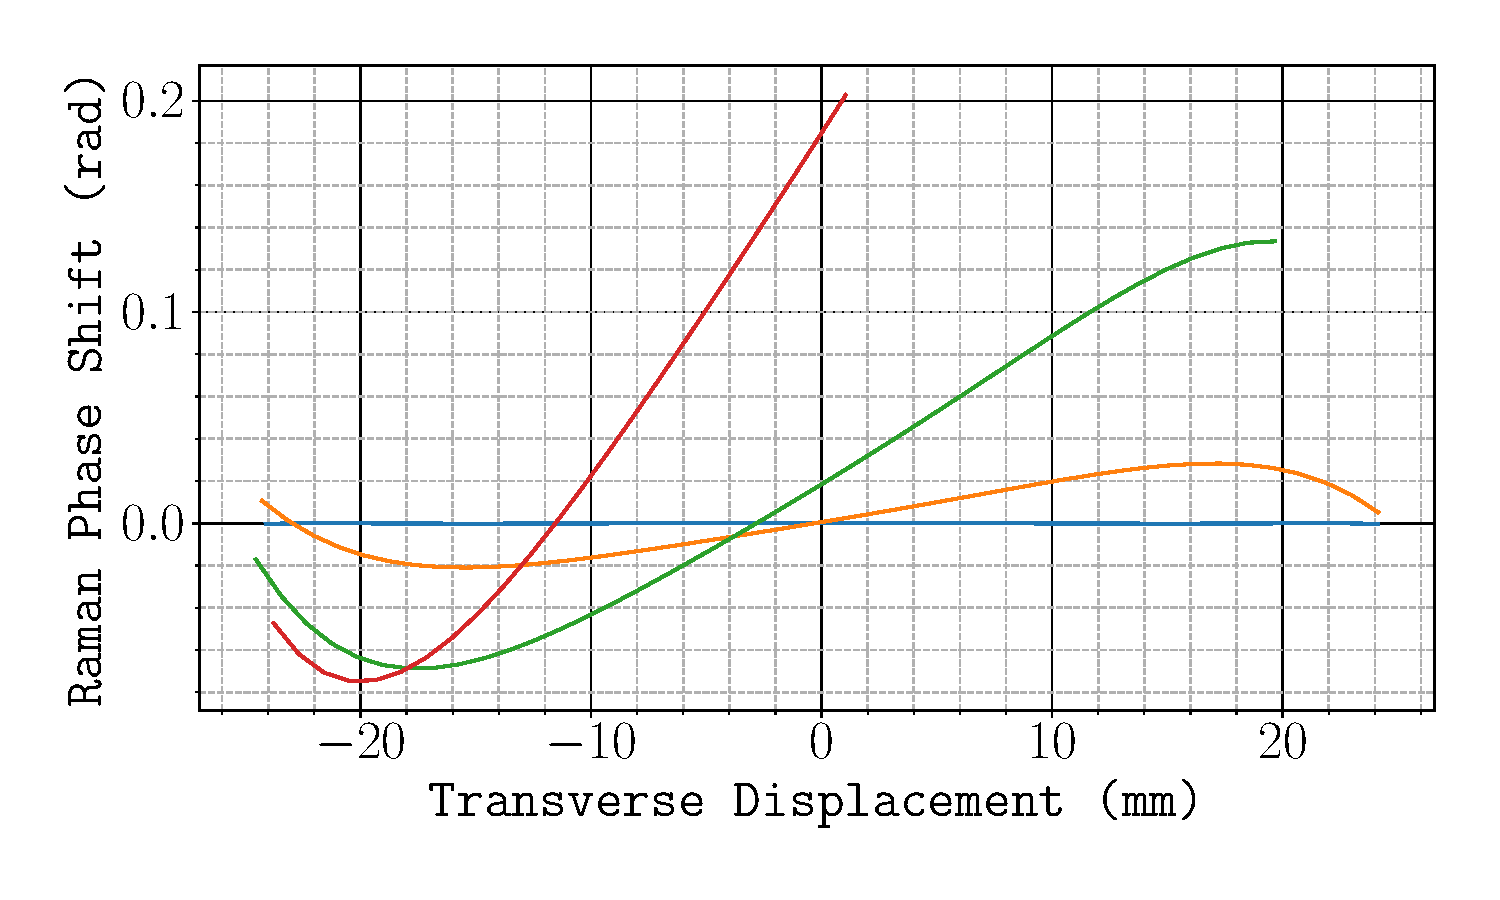
\includegraphics[width=0.4\textwidth]{wavefront_transverse.pdf}\label{fig:raman_wave_transverse}}
	\subfloat[][]{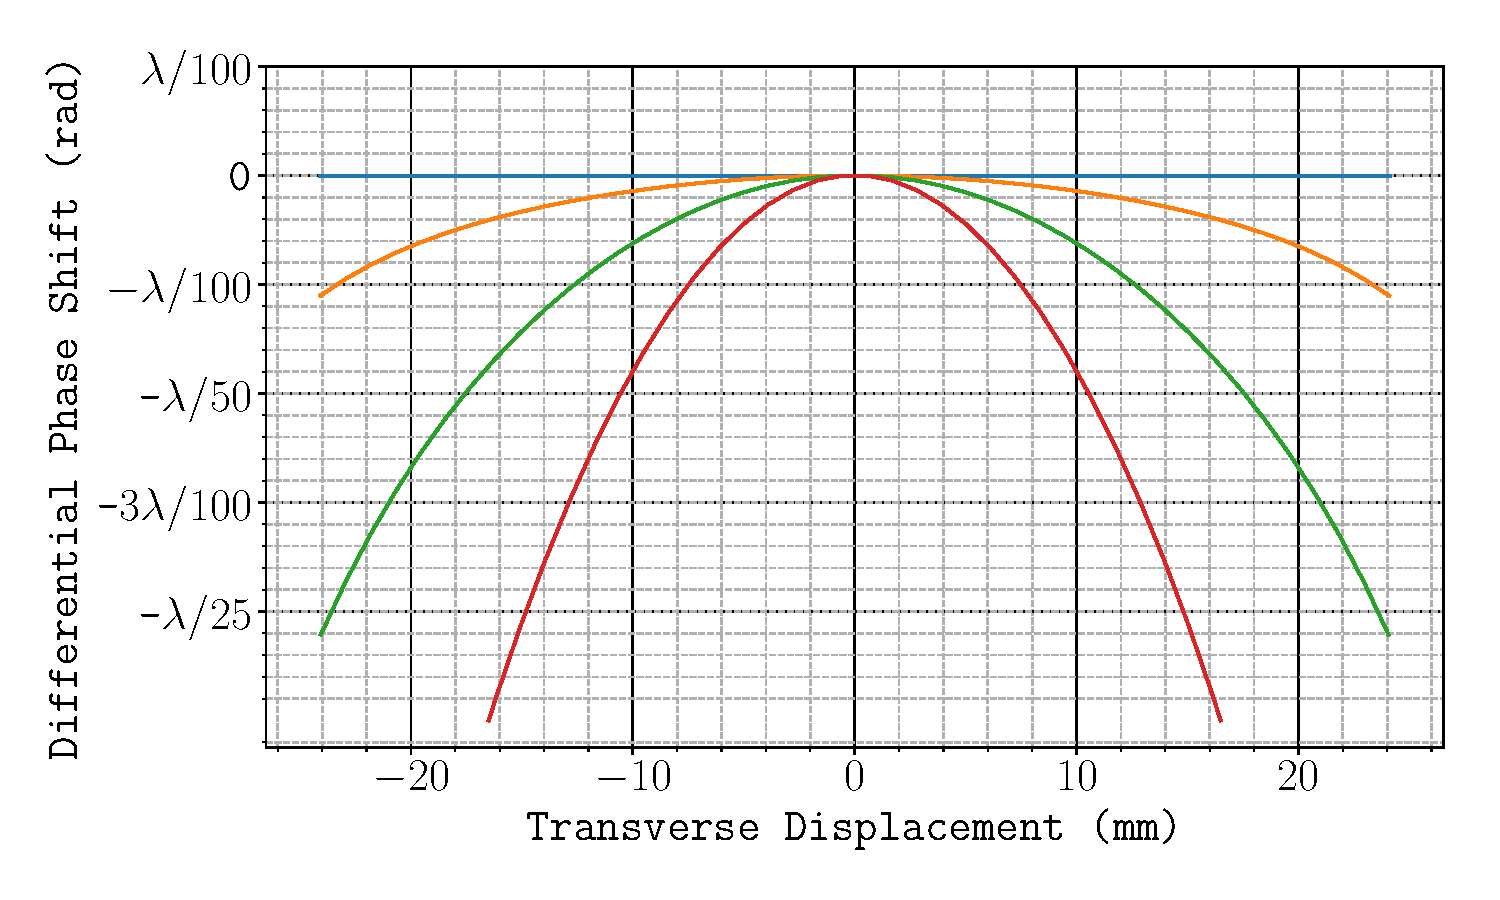
\includegraphics[width=0.4\textwidth]{wavefront_longitudinal.pdf}\label{fig:raman_wave_longitudinal}}
	\caption[Simulated wavefront distortion for longitudinal and transverse fibre
		misalignment]{Simulated wavefront distortion for longitudinal and transverse
		fibre misalignment. Rays from a point source with a divergence angle
		corresponding to a \ac{na} of 0.12 are propagated through the Raman optical
		system. Rays corresponding to the reflected beam are propagated further with
		the assumption that the mirror is perpendicular to the optic axis. The first
		set of rays propagates \sivalue{43}{\milli\metre} and the second propagates
		\sivalue{129}{\milli\metre}. The wavefront for each beam is calculated by
		taking the slope of each ray and subtracting from the slope of the central
		ray. The wavefront of the effective field that drives the Raman transition is
		the difference of these two wavefronts. (a) shows the distortion of the
		wavefront for a transverse misalignment of the fibre for a displacement of
		\sivalue{0}{\milli\metre} (blue), \sivalue{0.5}{\milli\metre} (orange)
		\sivalue{1}{\milli\metre} (green) and \sivalue{1.5}{\milli\metre} (red) from
		the front focal point. (b) shows the wavefront for longitudinal displacements
		of \sivalue{0}{\milli\metre} (blue), \sivalue{0.3}{\milli\metre} (orange)
		\sivalue{0.6}{\milli\metre} (green) and \sivalue{1}{\milli\metre}
		(red).}\label{fig:fig_label}
\end{figure}
\subsubsection{Measuring the Beam Width and Divergence}
Most of the characterisation of the beam was taken outside of the vacuum
chamber, prior to installation, due to extra difficulties of measuring its
properties \textit{in situ}. To measure the beam waist as well as its
divergence, the beam was used to illuminate a piece of paper aligned
perpendicular to the optic axis. This was then imaged using a CCD camera with
an objective lens so the entire spatial extent of the beam could be imaged.
The camera was calibrated to give an effective pixel size of
\sivalue{5.1}{pix/\milli\metre}. Both the camera and paper were mounted on a
translation stage, so that they could be moved along the direction of
propagation. This

\subsection{Retro-reflection Assembly}\label{subsec:setup_ramanmirror}
The mirror, also manufactured by Light Machinery, that is used to
retro-reflect the incoming beams is mounted on the opposite side of the
chamber. In order to drive Raman transitions
(see~\SectionRef{sec:raman_transitions} for further detail) with
counter-propagating light fields, a second \ac{qwp}, made to the same
specifications as the one in front of the collimation optics, is mounted in
front of the mirror. If the forward-propagating fields are circularly
polarised, the reflected ones will be polarised with the same handedness
regardless of the orientation of this second \ac{qwp}. \par\noindent
During the manufacturing process, the waveplates and mirror were polished to
reduce irregularities in the thickness of each \ac{qwp} and the surface of
the mirror. \FigureRef{fig:waveplate_map} shows the variation in the
thickness of the waveplate in front of the triplet lens, measured by Light
Machinery using a white light interferometer. This has a standard deviation
of \sivalue{4.62}{\nano\metre} and corresponds a standard deviation of the
optical path length of \pow{8.6}{-3}\(\lambda\).
\begin{figure}
	\centering
	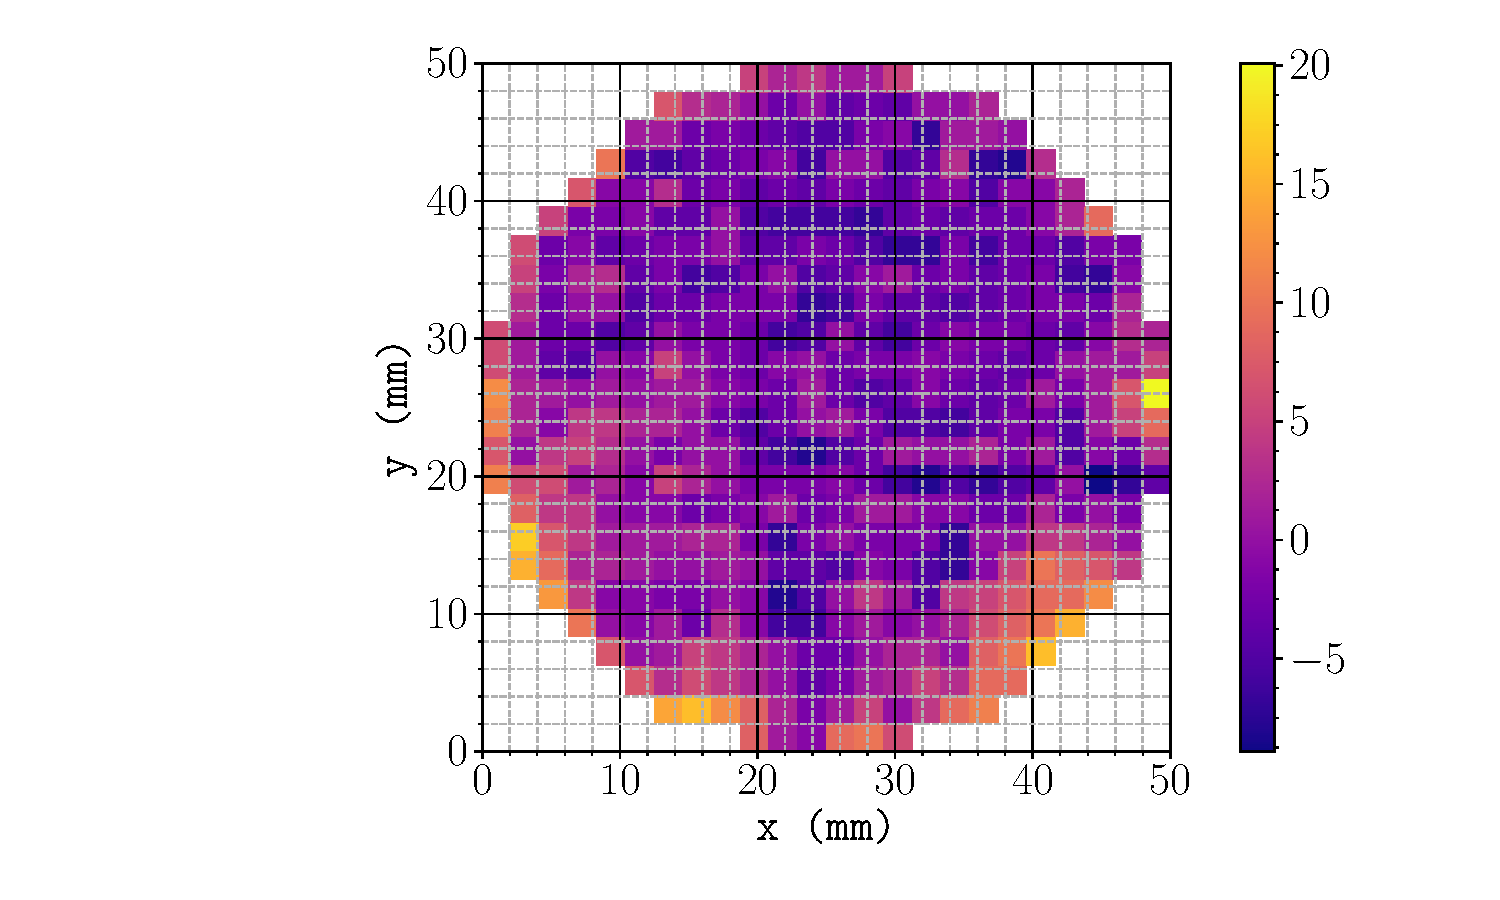
\includegraphics[width=0.5\textwidth]{waveplate.pdf}
	\caption{Thickness of the first \ac{QWP}, measured by a white light
		interferometer. The value is given in \sivalue{}{\nano\metre} as a difference
		from the mean thickness. The standard deviation of this thickness is
		\sivalue{4.62}{\nano\metre} and a peak-to-valley (PV) of {\textbf need number
				here}. Equivalent surface data for the other \ac{QWP} and mirror were not
		provided by Light Machinery, but had a PV thickness variation of
		\sivalue{19}{\nano\metre} and \sivalue{9}{\nano\metre} respectively.}
	\label{fig:waveplate_map}
\end{figure}
\par\noindent
The \ac{qwp} and mirror are fixed onto the front plate of a UHV compatible
MDI-HS mirror mount, manufactured by Radiant dye. The horizontal and vertical
tilt of the mirror can be adjusted using two thumbscrew actuators which cause
the front plate to pivot around a ball bearing. This mount is designed for
applications which require high stability, but of course the alignment will
still drift over time. To avoid the need to periodically open the chamber to
realign the mirror, a piezo-electric stack is placed between each actuator
and the front plate so that the tilt of the mirror can be adjusted
externally. Each piezo-stack is connected to a high-voltage feedthrough, so
that their length (and hence mirror tilt) can be finely adjusted by
controlling the voltage applied across them. A control voltage ranging
between 0--\sivalue{10}{\volt} is amplified by a controller to give an
applied voltage across the piezo stack that ranges between
-10--\sivalue{150}{\volt}, corresponding to a travel range of
\sivalue{23}{\micro\metre}.
\par\noindent
To understand the effect of misalignment, it is instructive to consider its
effect on the effective wavevector \(\keff\). As illustrated in
\FigureRef{fig:retro_misalign}, if the mirror is misaligned from the incoming
beam's wavevector by an angle \(theta\), the two counter-propagating fields
that drive Raman transitions have wavevectors \(k_1 \left(1,0\right)\) and
\(k_2 \left(\cos(\theta),\sin(\theta)\right)\). \(\keff = {\textbf k_1} -
{\textbf k_2} \cos (2\theta_i)\). Fortunately, for small angular
displacements, i.e. \(< \sivalue{1}{\milli\radian}\), this does not greatly
reduce the sensitivity to accelerations. In short, this means that \(\keff\)
will have a spatially varying direction. Since an atom interacting via a
Raman transition picks up a phase \(\phi = \keff . {\textbf x}\), atoms
travelling along different trajectories will accumulate different phases due
to the spatial variation of \(\keff{}\). Across the atom ensemble, this leads
to a dephasing and consequently, a loss of interferometer fringe
visibility~\cite{Tackmann2012}
\subsubsection{In-Situ Alignment and Optimisation}
After mounting the Raman optical system inside the chamber, the mirror had to
be aligned to retro-reflect the light. When the mirror is close to
perpendicular to the light's wavevector, some of the power in the reflected
beam couples back into the fibre. In principle, this power is maximised when
the mirror is exactly perpendicular so maximising this power is a useful
technique to align the mirror. A 99:1 fibre splitter was used to couple light
into the chamber, which provided a means to measure the back-reflected power
without needing any free-space optics. This was set up so that 99\% of the
incoming light entered the chamber, with the other 1\% coupled into the
corresponding output port. Due to the fact that a beam-splitter acts
reversibly, 1\% of the back-reflected light which couples into vacuum fibre
exits the fibre-splitter on the other input port. Therefore, the power at
this output was used to indirectly measure the alignment of the mirror.
\par\noindent
Since the travel range of the piezo stacks does not cover the full motional
range of the mirror mount, the mirror initially had to be manually aligned
using the thumbscrew actuators. Once installed, the lack of direct access to
optical system meant that conventional methods to coarsely align the mirror,
such as observing the location of the reflected beam's focus, were not
feasible. Rather than carry out the somewhat tedious job of systematically
adjusting each thumbscrew until the mirror was aligned, an automatic routine
was devised to do this. This was carried out using a pair of bipolar stepper
motors that each rotated a ball driver inserted into the head of each
thumbscrew. The revolution of these motors was controlled using an arduino
microcontroller, which communicated to the computer using a serial interface.
The motors rotated by 0.9\(\deg\)/step, which corresponds to a tilt of the
mirror by \sivalue{18.1}{\micro\radian}. This is smaller than the
\sivalue{0.67}{\milli\radian} angular displacement that the piezo stack could
provide, but the slow execution speed of the motor control meant that it was
more practical to use a combination of the motors and piezos to
systematically scan through the tilt of the mirror mount.
{\textbf {huge find out how big spot size was }}. \par\noindent
Using this method, the mirror mount was aligned so that the the maximum of
the back-reflected power was reachable with the piezo stacks. Of course, it
was forseeable that the mirror would need to be periodically realigned, which
would require another systematic iteration through the voltages applied to
each piezo stack. Given that this search was quite time consuming, it was not
a practical way to maintain alignment. To improve upon this, an optimisation
method using the Nelder-Mead simplex algorithm~\cite{Nelder1965} was
implemented. This method is suitable for optimising multidimensional
functions and has been used to demonstrate the automatic alignment of a fibre
with up to 6 degrees of freedom~\cite{Zhang2004}. In general terms, this
algorithm aims to optimise the value of an objective function (in this
instance, the optical power measured as a voltage by a photodiode) by
sampling the function at various locations. For \(n\) parameters, a set of
\(n-1\) points distributed randomly across the parameter space are chosen as
the initial simplex. These are sorted in decreasing order of the value of the
obejctive function and the algorithm proceeds by performing geometric
transformations on this simplex, by sequentially reflecting, expanding and
contracting this simplex. Each step starts with a reflection about the line
between the two greatest values. The coordinates of the simplex are updated
if the function has a greater value at the location given by one of these
transformations, until the algorithm converges on a maximum value. As with
many optimisation algorithms, the Nelder-Mead method has the potential to
converge on a local optimum, but this is allieviated by expanding the simplex
to look for more optimal values. The termination of the algorithm was decided
by using the standard deviation of the last 5 values. Empirically, it was
found that terminating when the standard deviation was less than
\sivalue{10}{\micro\volt} resulted in stable performance of the algorithm,
even when the signal-to-noise ratio of the measured voltage was poor. An
example of this algorithm aligning the mirror mount is presented in
\FigureRef{fig:simplex_optimisation}. To verify that the converged value was
optimal, a systematic scan of the piezo stack control voltages in the region
around this value was also carried out. In this case, the algorithm converged
on a local maximum, but one that greatly enhanced the coupling efficiency of
the reflected light back into the fibre. The difference in the piezo control
voltages from their optimal values corresponds to a tilt of the mirror mount
along the horizontal and vertical axis of less than
\sivalue{13}{\micro\radian}.
\begin{figure}
	\centering
	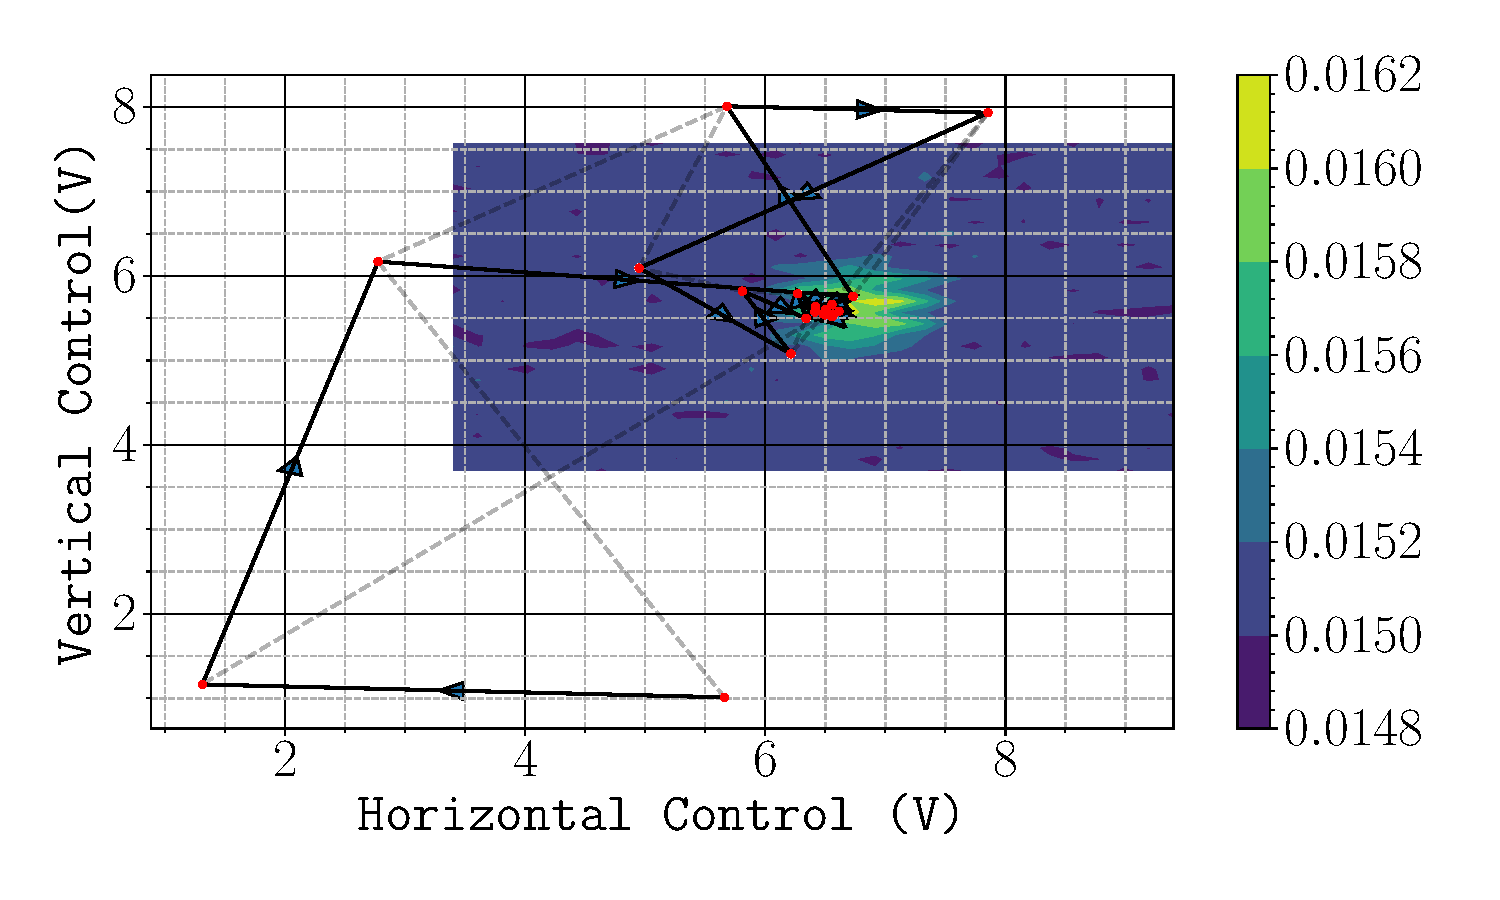
\includegraphics[width=0.5\textwidth]{simplex_alignment}
	\caption[Automatic mirror alignment using the Nelder-Mead simplex
		algorithm.]{Automatic mirror alignment using the Nelder-Mead simplex
		algorithm. This
		procedure starts by randomly selecting three pairs of control voltages for
		the horizontal and vertical piezo stacks. At each co-ordinate, the
		back-reflected power is measured. The algorithm proceeds by geometrically
		transforming the simplex using reflections, expansions and contractions, and
		updating the simplex using this new co-ordinate if the power measured is
		greater than the current lowest value. The algorithm uses the standard
		deviation of the last 5 values as a check for convergence. In this case, it
		terminates once the standard deviation is smaller than
		\sivalue{10}{\micro\volt}. The shaded lines indicate the simplex bounded by
		the three co-ordinates at each iteration, whose area reduces as the algorithm
		converges on the optimum value. A scan of the piezo control voltages close to
		the optimum is also plotted. The irregular shape of the measured power is a
		result of a hysteresis effect when the horizontal control voltage was changed
		from its maximum value to the minimum. Even with a low signal-to-noise ratio,
		the algorithm converged on a value close to the optimum. This resulted in a
		misalignment of less than \sivalue{13}{\micro\radian} along both axes.}
	\label{fig:simplex_optimisation}
\end{figure}
\subsection{The MEMS Accelerometer}\label{subsec:raman_mems}

\section{Driving Raman Transitions}\label{sec:raman_transitions}
As the forward-propagating fields have opposite handedness, the counter-propagating fields have the same handedness as the field
\subsection{Frequency and Phase Control}\label{subsec:msquared_comm}

\section{Atom Detection}
\subsection{Optical System}\label{subsec:photodiode_setup}
\subsection{Measuring the Interferometer Phase}

\section{Individual Pulse Characterisation} \label{sec:atomint_rabiosc}
\subsection{Velocity-Selective Pulse}
\subsection{Interferometer Pulses}

\section{Three-Pulse Atom Interference} \label{sec:atomint_threepulse}
\subsection{Fringe Contrast vs. Launch Trajectory}\label{subsec:launch_contrast}
\section{Measuring Accelerations}\label{sec:atomint_accelerations}
\subsection{Vibration Sensitivity}
